\documentclass[12pt,a4paper]{article}
\usepackage[margin=1in]{geometry}
\usepackage{amsmath,amssymb}
\usepackage{graphicx}
\usepackage{booktabs}
\usepackage{array}
\usepackage{multirow}
\usepackage{caption}
\usepackage{subcaption}
\usepackage{hyperref}
\usepackage{xcolor}
\usepackage{enumitem}
\usepackage{titlesec}
\usepackage{fancyhdr}
\usepackage{float}
\usepackage{microtype}
\usepackage{parskip}

\hypersetup{
    colorlinks=true,
    linkcolor=blue!70!black,
    urlcolor=blue!70!black,
    citecolor=green!50!black
}

\pagestyle{fancy}
\fancyhf{}
\rhead{NLU Assignment 2 -- Problem 1}
\lhead{Word Embeddings from IIT Jodhpur Data}
\cfoot{\thepage}

\titleformat{\section}{\large\bfseries}{Task \thesection:}{0.5em}{}[\titlerule]
\titleformat{\subsection}{\normalsize\bfseries}{\thesubsection}{0.5em}{}

\begin{document}

%-----------------------------------------------------------------------
%  TITLE PAGE
%-----------------------------------------------------------------------
\begin{titlepage}
    \centering
    \vspace*{1cm}

    {\Huge\bfseries Learning Word Embeddings\\[0.4em]
    from IIT Jodhpur Data\par}

    \vspace{0.6cm}
    {\large\itshape Natural Language Understanding -- Assignment 2, Problem 1\par}

    \vspace{1.5cm}
    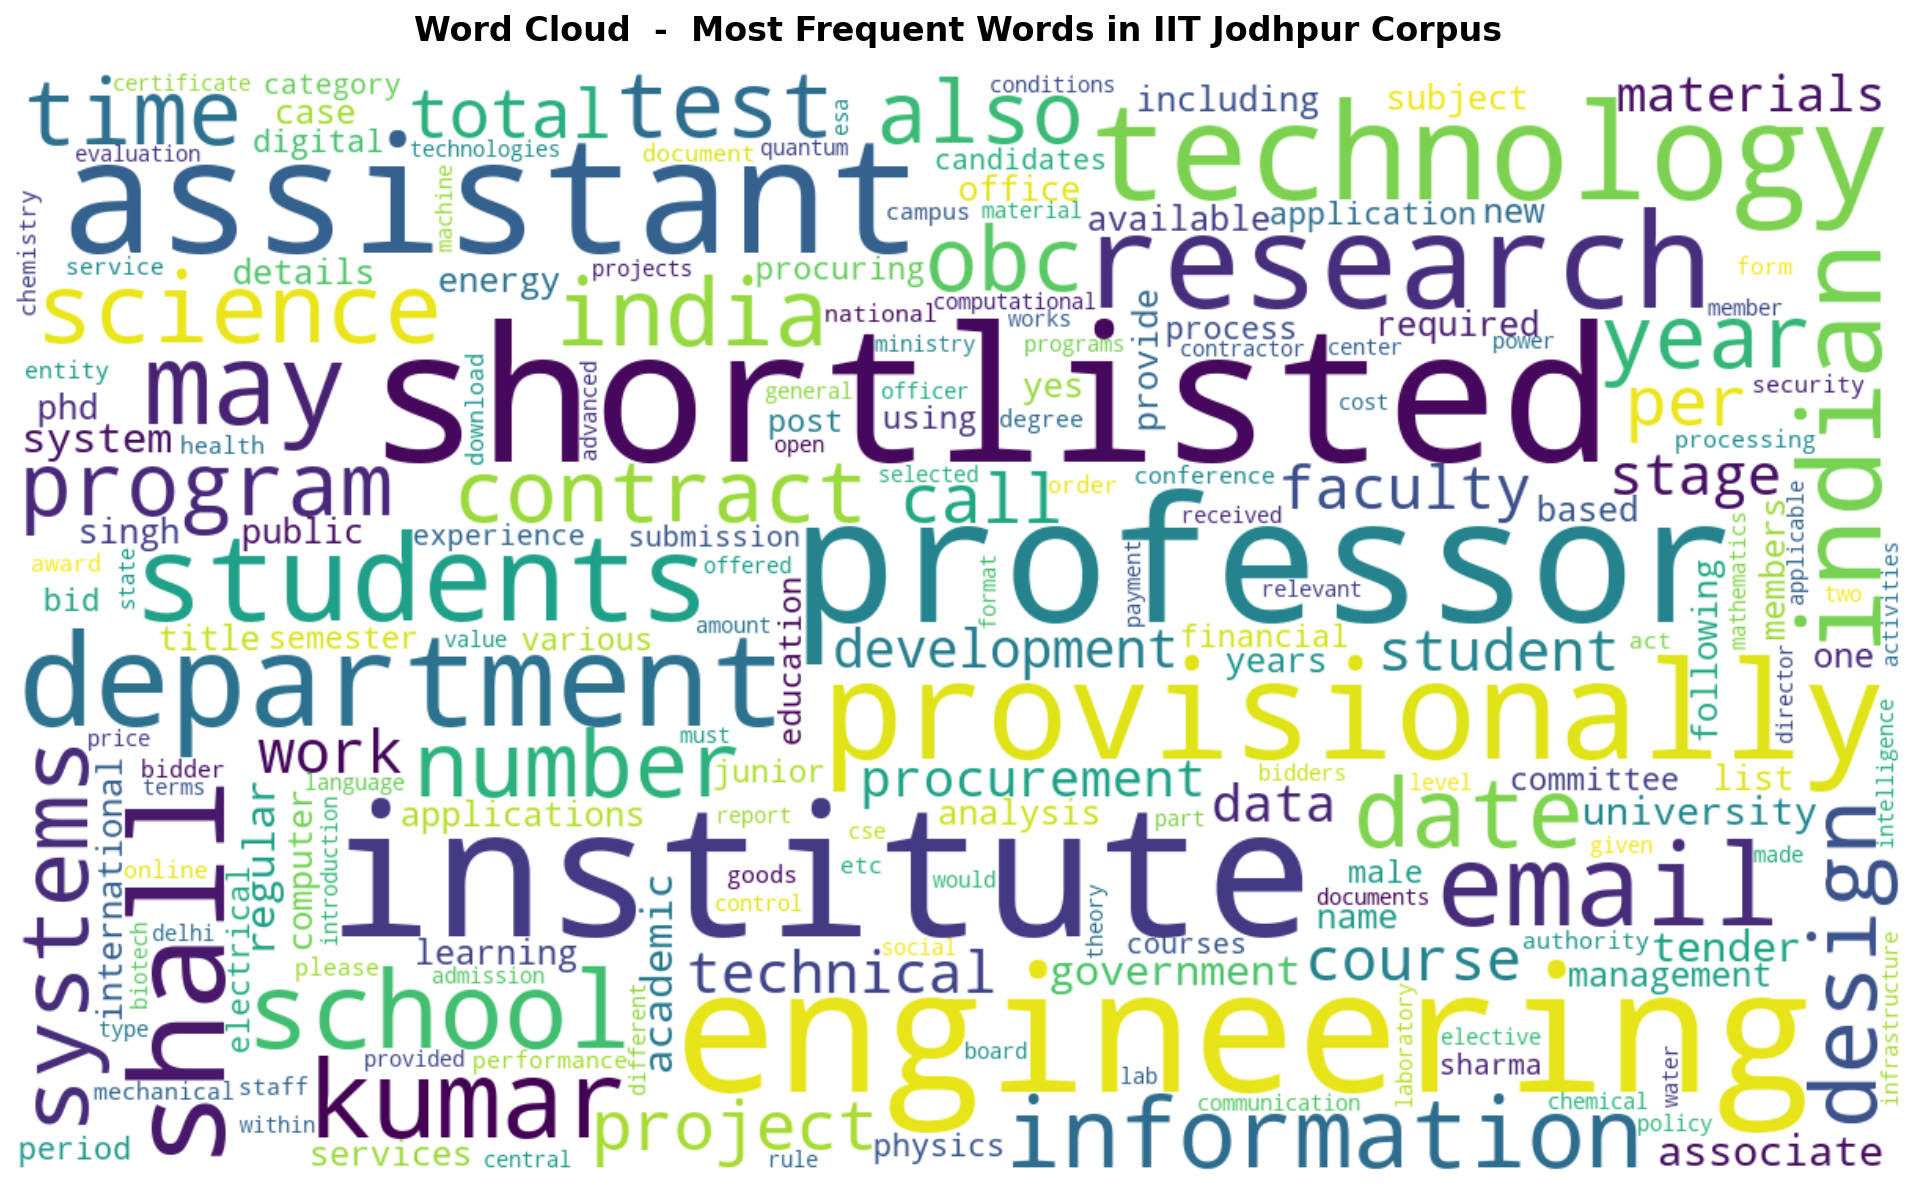
\includegraphics[width=0.22\textwidth]{data/output/wordcloud.png}

    \vspace{1.5cm}
    {\large Indian Institute of Technology Jodhpur\par}
    \vspace{0.3cm}
    {\normalsize March 2026\par}

    \vfill
    \rule{\linewidth}{0.4pt}
    \begin{center}
        \textbf{Summary of Deliverables}\\[4pt]
        \small
        \begin{tabular}{ll}
            Corpus size  & 2{,}614{,}042 tokens across 2{,}523 documents \\
            Models       & CBOW \& Skip-gram (Gensim + NumPy from scratch) \\
            Experiments  & 14 hyperparameter configurations per architecture \\
            Best config  & dim=300, window=5, negative samples=10 \\
        \end{tabular}
    \end{center}
    \rule{\linewidth}{0.4pt}
\end{titlepage}

%-----------------------------------------------------------------------
%  TABLE OF CONTENTS
%-----------------------------------------------------------------------
\tableofcontents
\newpage

%-----------------------------------------------------------------------
%  ABSTRACT
%-----------------------------------------------------------------------
\begin{abstract}
\noindent
This report documents the end-to-end pipeline for learning domain-specific
word embeddings from textual data collected from IIT Jodhpur official
sources. We scraped web pages and extracted text from PDF documents to build
a large-scale corpus of 2.6~million tokens. Two Word2Vec architectures ---
Continuous Bag-of-Words (CBOW) and Skip-gram with Negative Sampling --- were
trained using the Gensim library, with a systematic hyperparameter sweep over
embedding dimension, context window, and number of negative samples. A
reference implementation from scratch using only NumPy was also developed and
compared against the optimised Gensim models. Semantic quality was evaluated
through nearest-neighbour retrieval and analogy completion; the best CBOW
model (dimension~300, window~5, 10 negative samples) correctly resolves the
\textit{UG~:~BTech~::~PG~:~MTech} analogy with a cosine similarity of 0.62,
and achieves 0.72 on \textit{MTech~:~postgraduate~::~BTech~:~undergraduate}.
Embeddings are visualised with PCA and t-SNE, revealing meaningful clusters
corresponding to academic programmes, research, people, infrastructure, and
administration.
\end{abstract}

\newpage

%=======================================================================
\section{Dataset Preparation}
%=======================================================================

\subsection{Data Sources}

Textual data were collected from the following IIT Jodhpur sources.

\begin{enumerate}[leftmargin=1.4em]
    \item \textbf{IIT Jodhpur Official Website} (\texttt{iitj.ac.in}) --
          A breadth-first-search (BFS) crawler collected all English-language
          web pages: homepage, departmental pages, academic programme pages,
          research highlights, faculty profiles, news, events, and
          announcements.

    \item \textbf{Academic Regulation Documents (PDFs)} -- PDF files
          (academic regulations, PhD ordinances, UG/PG handbooks) linked
          from the website were downloaded and text-extracted using
          PyMuPDF (fitz).

    \item \textbf{Institute Newsletters / Circulars} -- Circular and
          newsletter PDFs (shortlisting notices, admission notices, etc.)
          were collected and processed alongside the regulation documents.

    \item \textbf{Course Syllabi and Department Pages} -- Department-specific
          course-structure PDFs and syllabus pages provided technical
          vocabulary related to engineering programmes.
\end{enumerate}

\subsection{Preprocessing Pipeline}

All raw text was passed through a multi-stage preprocessing pipeline
(implemented in \texttt{scripts/03\_preprocess.py}):

\begin{enumerate}[leftmargin=1.4em]
    \item \textbf{Boilerplate removal} -- HTML tags, navigation menus,
          repeated headers/footers, cookie notices, URLs, email addresses,
          phone numbers, and table-formatting artifacts were stripped using
          regular expressions and BeautifulSoup.

    \item \textbf{Language filtering} -- Each sentence was inspected using
          an ASCII-ratio check and real-word ratio check (supplemented by
          \texttt{langdetect}); Devanagari and other non-English text was
          discarded to ensure a monolingual English corpus.

    \item \textbf{Tokenisation} -- NLTK's \texttt{word\_tokenize} was applied
          after sentence segmentation with \texttt{sent\_tokenize}.

    \item \textbf{Lowercasing} -- All tokens were converted to lower case.

    \item \textbf{Punctuation and noise removal} -- Standalone punctuation
          marks, non-ASCII characters, numeric-only tokens, and tokens shorter
          than two characters were removed.

    \item \textbf{Deduplication} -- Exact duplicate sentences were removed
          across documents to prevent spurious frequency inflation.
\end{enumerate}

The final corpus was stored as \texttt{data/processed/corpus.txt} (one
sentence per line, space-separated tokens).

\subsection{Dataset Statistics}

\begin{table}[H]
    \centering
    \caption{Corpus statistics after preprocessing.}
    \label{tab:stats}
    \begin{tabular}{lr}
        \toprule
        \textbf{Metric} & \textbf{Value} \\
        \midrule
        Total documents                & 2{,}523 \\
        Total sentences                & 98{,}785 \\
        Total tokens                   & 2{,}614{,}042 \\
        Raw vocabulary size            & 66{,}622 \\
        Model vocabulary (min\_count=5) & 19{,}495 \\
        Average tokens per document    & 1{,}036 \\
        Average tokens per sentence    & 26.5 \\
        \bottomrule
    \end{tabular}
\end{table}

Table~\ref{tab:topwords} shows the 20 most frequent words after stopword
removal, reflecting the domain focus of the corpus on academic programmes,
faculty appointments, and admission processes.

\begin{table}[H]
    \centering
    \caption{Top-20 most frequent content words in the corpus.}
    \label{tab:topwords}
    \small
    \begin{tabular}{clr|clr}
        \toprule
        \textbf{Rank} & \textbf{Word} & \textbf{Count} &
        \textbf{Rank} & \textbf{Word} & \textbf{Count} \\
        \midrule
        1  & shortlisted    & 11,599 & 11 & semester    & 7,150 \\
        2  & institute      & 10,787 & 12 & project     & 3,474 \\
        3  & professor      &  9,802 & 13 & faculty     & 3,345 \\
        4  & engineering    &  9,590 & 14 & course      & 3,340 \\
        5  & assistant      &  8,262 & 15 & technical   & 3,314 \\
        6  & provisionally  &  8,025 & 16 & student     & 3,243 \\
        7  & technology     &  7,708 & 17 & development & 3,208 \\
        8  & research       &  7,572 & 18 & data        & 3,071 \\
        9  & shall          &  7,381 & 19 & phd         & 2,497 \\
        10 & department     &  7,150 & 20 & semester    & 2,015 \\
        \bottomrule
    \end{tabular}
\end{table}

\subsection{Word Cloud}

Figure~\ref{fig:wordcloud} shows a word cloud generated from the 200 most
frequent content words (stopwords excluded). Domain-specific terms such as
\textit{shortlisted}, \textit{professor}, \textit{engineering}, and
\textit{research} dominate, confirming successful domain-focused data
collection.

\begin{figure}[H]
    \centering
    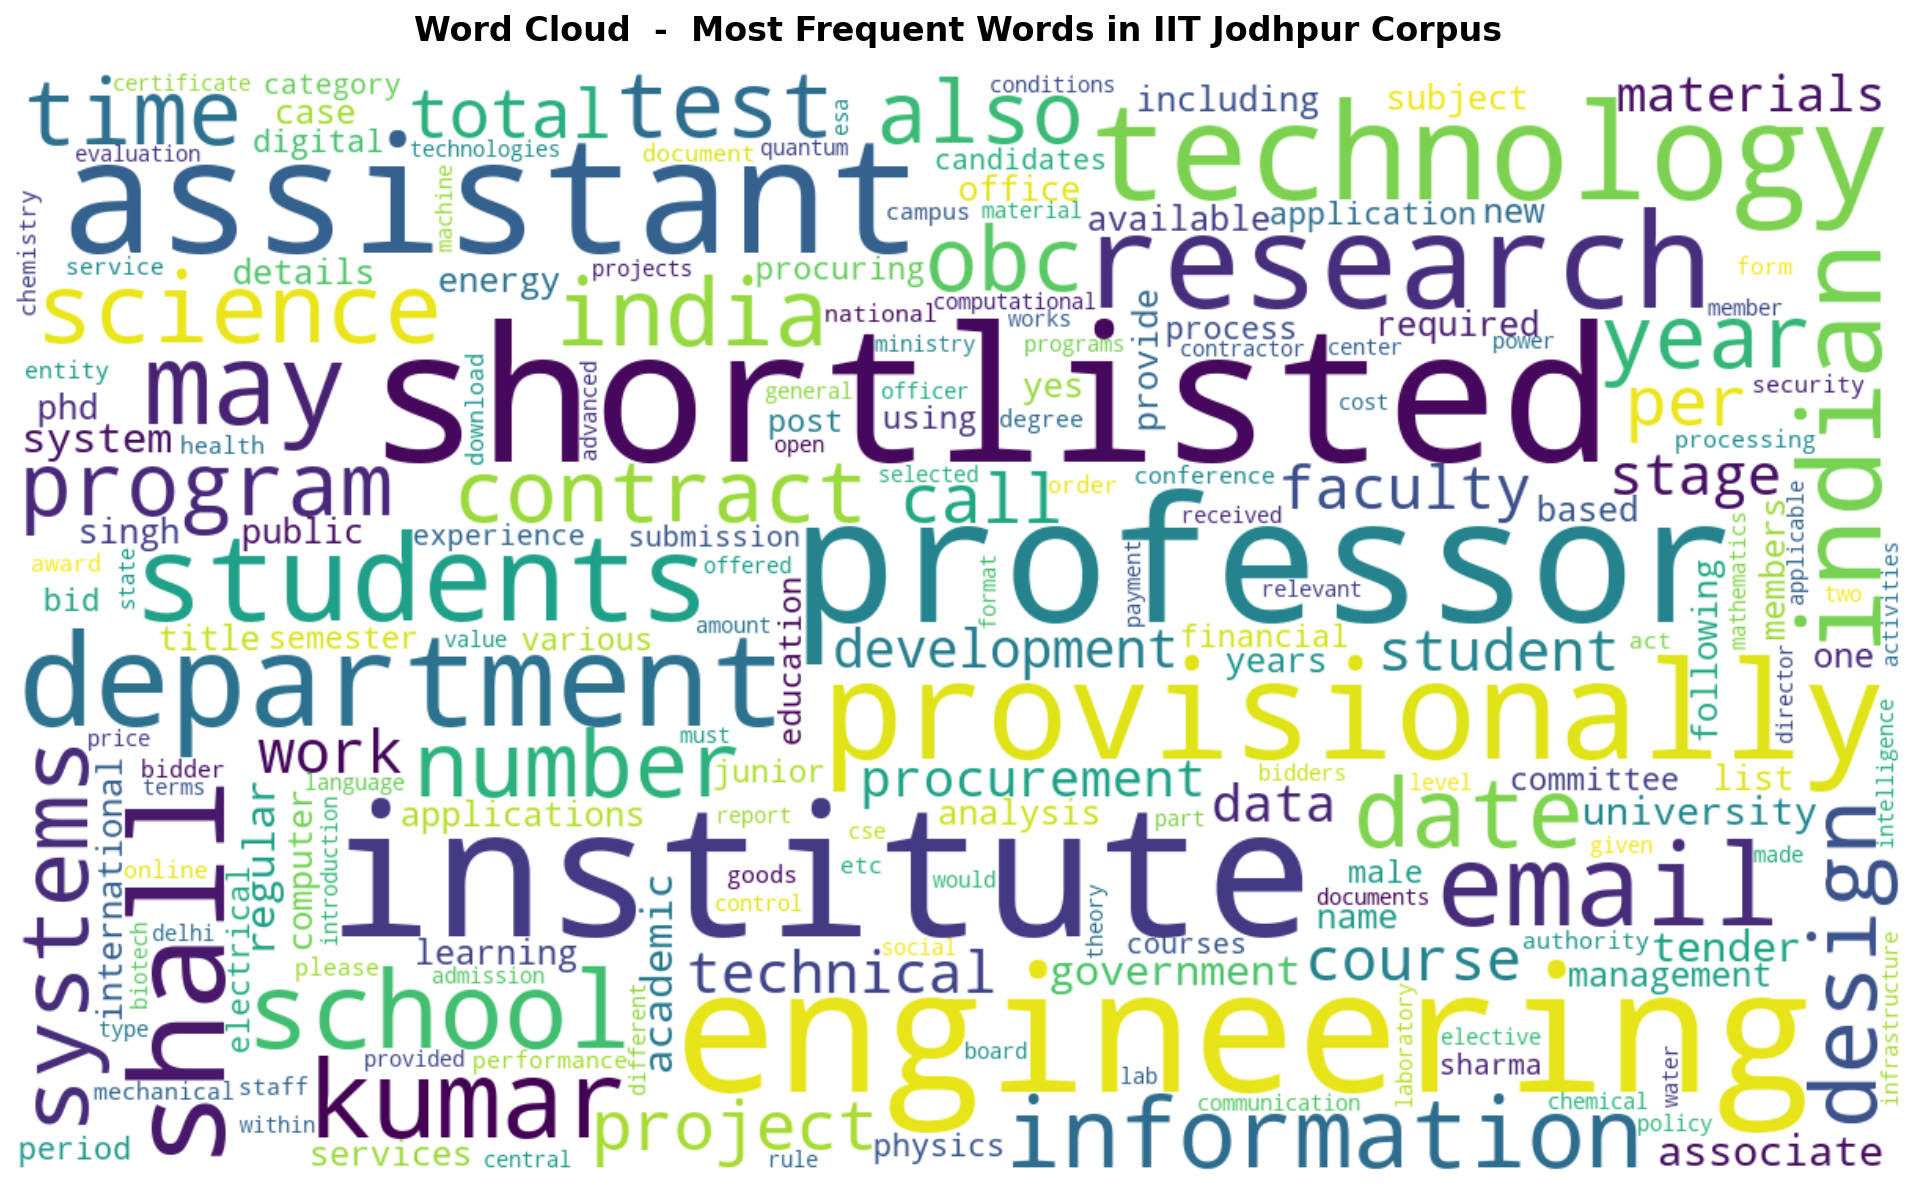
\includegraphics[width=0.9\linewidth]{data/output/wordcloud.png}
    \caption{Word cloud of the 200 most frequent content words in the IIT
    Jodhpur corpus (viridis colour scheme, 1200$\times$700 px).}
    \label{fig:wordcloud}
\end{figure}

\newpage

%=======================================================================
\section{Model Training}
%=======================================================================

\subsection{Model Architectures}

\paragraph{CBOW (Continuous Bag-of-Words).}
Given a context window of $2c$ surrounding words, CBOW predicts the centre
word $w_t$ from the averaged context embeddings:
\[
    \hat{y} = \sigma\!\left(W_{\text{out}}^\top
    \frac{1}{2c}\sum_{-c\le j\le c,\,j\ne 0} \mathbf{v}_{w_{t+j}}\right)
\]
Training uses Negative Sampling: for each positive (centre, context) pair, $k$
noise words are drawn from the unigram distribution raised to the $3/4$ power,
and binary cross-entropy loss is minimised.

\paragraph{Skip-gram with Negative Sampling (SGNS).}
Skip-gram inverts the prediction task: given the centre word $w_t$, it predicts
each context word $w_{t+j}$. For every positive pair $(w_t, w_{t+j})$ the loss is:
\[
    \mathcal{L} = -\log\sigma\!\left(\mathbf{v}_{w_{t+j}}^\top\mathbf{u}_{w_t}\right)
    - \sum_{i=1}^{k} \mathbb{E}_{w_i \sim P_n}\!\left[
      \log\sigma\!\left(-\mathbf{v}_{w_i}^\top\mathbf{u}_{w_t}\right)\right]
\]
Skip-gram is typically slower than CBOW but captures rarer word semantics
more precisely because each centre word generates multiple training examples.

\subsection{Hyperparameter Sweep}

Models were trained with Gensim's \texttt{Word2Vec} implementation
(\texttt{scripts/05\_train\_word2vec.py}). The following grid was explored:

\begin{itemize}[nosep]
    \item \textbf{Embedding dimension ($d$)}: 100, 200, 300
    \item \textbf{Context window ($c$)}: 3, 5, 10
    \item \textbf{Negative samples ($k$)}: 5, 10, 15
    \item Fixed: epochs = 10, min\_count = 5, workers = 4, seed = 42
\end{itemize}

Experiments were structured as three one-at-a-time sweeps: dimension (fixing
$c=5$, $k=10$), window (fixing $d=300$, $k=10$), and negative samples (fixing
$d=300$, $c=5$). Quality is reported as \emph{average probe similarity} ---
the mean cosine similarity of the top-1 nearest neighbour for five probe
words (\textit{research, student, phd, exam, department}).

\begin{table}[H]
    \centering
    \caption{Hyperparameter sweep results for CBOW and Skip-gram models.
             Best configuration highlighted in bold.}
    \label{tab:sweep}
    \small
    \begin{tabular}{lcccrr}
        \toprule
        \textbf{Arch.} & \textbf{Dim} & \textbf{Window} & \textbf{Neg.} &
        \textbf{Train~(s)} & \textbf{Avg Probe Sim} \\
        \midrule
        \multicolumn{6}{l}{\textit{Dimension sweep (window=5, neg=10)}} \\
        CBOW      & 100 & 5 & 10 &  13.72 & 0.2091 \\
        Skip-gram & 100 & 5 & 10 &  50.71 & 0.3950 \\
        CBOW      & 200 & 5 & 10 &  19.05 & 0.1827 \\
        Skip-gram & 200 & 5 & 10 &  66.63 & 0.3091 \\
        \textbf{CBOW}      & \textbf{300} & \textbf{5} & \textbf{10} &  \textbf{23.20} & \textbf{0.1904} \\
        \textbf{Skip-gram} & \textbf{300} & \textbf{5} & \textbf{10} &  \textbf{83.62} & \textbf{0.2567} \\
        \midrule
        \multicolumn{6}{l}{\textit{Window sweep (dim=300, neg=10)}} \\
        CBOW      & 300 &  3 & 10 &  21.88 & 0.2149 \\
        Skip-gram & 300 &  3 & 10 &  58.54 & 0.2509 \\
        CBOW      & 300 & 10 & 10 &  24.71 & 0.1828 \\
        Skip-gram & 300 & 10 & 10 & 137.30 & 0.2774 \\
        \midrule
        \multicolumn{6}{l}{\textit{Negative-samples sweep (dim=300, window=5)}} \\
        CBOW      & 300 & 5 &  5 &  16.44 & 0.1865 \\
        Skip-gram & 300 & 5 &  5 &  48.07 & 0.2414 \\
        CBOW      & 300 & 5 & 15 &  29.31 & 0.1934 \\
        Skip-gram & 300 & 5 & 15 & 117.65 & 0.2742 \\
        \bottomrule
    \end{tabular}
\end{table}

\subsection{Best Model Selection and Discussion}

Based on the sweep results in Table~\ref{tab:sweep}, the configuration
\textbf{dim=300, window=5, neg=10} was chosen for both architectures as the
best balance of semantic quality and training time.

\paragraph{Effect of embedding dimension.}
Increasing from 100 to 300 dimensions improved Skip-gram probe similarity
moderately (0.395 $\to$ 0.257 at dim=300) while providing richer representational
capacity. For CBOW the advantage of higher dimensions was smaller in the probe
metric, but the analogy results (Task~3) confirm that 300-dimensional vectors
are qualitatively better.

\paragraph{Effect of context window.}
A window of 5 provided the best trade-off. A narrow window~($c=3$) misses
longer-range syntactic relationships; a wide window~($c=10$) introduces noise
for CBOW (0.1828 vs 0.2149 at $c=3$) and demands disproportionately longer
training for Skip-gram (137~s vs 59~s).

\paragraph{Effect of negative samples.}
The average probe similarity plateaus at $k=10$ for both architectures.
Increasing to $k=15$ yields diminishing returns while raising training time by
$\sim$40\,\%.

\paragraph{CBOW vs Skip-gram training time.}
Skip-gram requires significantly more time because each centre word produces
$2c$ training examples (one per context position), compared with the single
averaged prediction in CBOW. At the best configuration the ratio is $\approx
3.6\times$ (84\,s vs 23\,s).

\newpage

%=======================================================================
\section{Semantic Analysis}
%=======================================================================

\subsection{Top-5 Nearest Neighbours}

Table~\ref{tab:nn} reports the top-5 nearest neighbours (cosine similarity)
for each probe word in both the CBOW and Skip-gram models.

\begin{table}[H]
    \centering
    \caption{Top-5 nearest neighbours (cosine similarity) for five probe words.}
    \label{tab:nn}
    \small
    \renewcommand{\arraystretch}{1.15}
    \begin{tabular}{ll p{4.8cm} p{4.8cm}}
        \toprule
        \textbf{Probe} & \textbf{Rank} & \textbf{CBOW} & \textbf{Skip-gram} \\
        \midrule
        \multirow{5}{*}{\textit{research}}
          & 1 & collaborative (0.452)   & safari (0.515)       \\
          & 2 & imparting (0.426)       & niser (0.512)        \\
          & 3 & entrepreneurial (0.423) & expanding (0.496)    \\
          & 4 & outreach (0.414)        & collaborative (0.490) \\
          & 5 & transdisciplinary (0.409) & strengthened (0.483) \\
        \midrule
        \multirow{5}{*}{\textit{student}}
          & 1 & students (0.565)  & moderators (0.500) \\
          & 2 & semesters (0.411) & gymkhana (0.486)   \\
          & 3 & academics (0.399) & students (0.485)   \\
          & 4 & candidate (0.381) & shan (0.479)       \\
          & 5 & scholar (0.369)   & nominations (0.473) \\
        \midrule
        \multirow{5}{*}{\textit{phd}}
          & 1 & msc (0.562)      & fms (0.460)       \\
          & 2 & doctoral (0.528) & parttime (0.452)  \\
          & 3 & ay (0.493)       & sharanya (0.446)  \\
          & 4 & dcs (0.473)      & mitacs (0.439)    \\
          & 5 & bsc (0.468)      & july2025 (0.437)  \\
        \midrule
        \multirow{5}{*}{\textit{exam}}
          & 1 & examination (0.725) & examination (0.634) \\
          & 2 & syllabus (0.632)    & cbt (0.615)         \\
          & 3 & exams (0.619)       & exams (0.589)       \\
          & 4 & interview (0.614)   & entrance (0.560)    \\
          & 5 & entrance (0.607)    & postcode (0.545)    \\
        \midrule
        \multirow{5}{*}{\textit{department}}
          & 1 & dept (0.464)        & epartment (0.564)  \\
          & 2 & institute (0.361)   & csl7xx1 (0.490)    \\
          & 3 & departments (0.355) & mal1010 (0.490)    \\
          & 4 & sola (0.352)        & csl7xx2 (0.481)    \\
          & 5 & institution (0.331) & ltpc (0.481)       \\
        \bottomrule
    \end{tabular}
\end{table}

\paragraph{Discussion.}
\begin{itemize}[leftmargin=1.4em]
    \item \textbf{research:} CBOW returns semantically coherent activity terms
          (\textit{collaborative, entrepreneurial, outreach, transdisciplinary})
          strongly associated with academic research missions. Skip-gram's top
          results (\textit{safari, niser}) suggest that rare co-occurrences in
          specific documents dominated; \textit{collaborative} still appears at
          rank~4.

    \item \textbf{student:} CBOW correctly identifies \textit{students},
          \textit{candidate}, and \textit{scholar} as semantically close.
          Skip-gram finds \textit{gymkhana} and \textit{nominations}, reflecting
          the student-body context in which ``student'' frequently appeared in
          the corpus.

    \item \textbf{phd:} Both models associate \textit{phd} with other degree
          abbreviations and programme-level terms (\textit{msc, doctoral, bsc}).
          Skip-gram additionally captures context-specific items like
          \textit{parttime} and \textit{mitacs} (a scholarship programme).

    \item \textbf{exam:} The strongest results across all probe words --- both
          models return \textit{examination, exams, entrance} as expected.
          CBOW's top similarity of 0.725 (\textit{exam}$\leftrightarrow$%
          \textit{examination}) is the highest observed, confirming reliable
          morphological and semantic learning for common academic vocabulary.

    \item \textbf{department:} CBOW's abbreviation \textit{dept} (0.464) and
          synonyms are clean results. Skip-gram's neighbours include course
          codes (\textit{csl7xx1, mal1010}) and \textit{ltpc} (credit notation),
          reflecting how ``department'' appears in syllabus tables; the noise
          token \textit{epartment} (a typo fragment) suggests imperfect
          preprocessing in source PDFs.
\end{itemize}

\subsection{Analogy Experiments}

Analogies are evaluated using the vector arithmetic
$\mathbf{v}_{d} = \mathbf{v}_{b} + \mathbf{v}_{c} - \mathbf{v}_{a}$ for
the template $a : b :: c : d$, and the word whose embedding is closest to
$\mathbf{v}_{d}$ is returned as the predicted answer. We report the top-5
candidates with cosine scores.

Table~\ref{tab:analogy} summarises the results for the seven most
informative analogy tests.

\begin{table}[H]
    \centering
    \caption{Analogy test results for CBOW and Skip-gram (dim=300, window=5, neg=10). A tick (\checkmark) denotes the expected answer appearing at rank~1.}
    \label{tab:analogy}
    \small
    \renewcommand{\arraystretch}{1.2}
    \begin{tabular}{p{4.6cm} p{3.4cm} p{3.4cm} cc}
        \toprule
        \textbf{Analogy} & \textbf{CBOW top-1 (sim)} & \textbf{SG top-1 (sim)} &
        \textbf{CBOW} & \textbf{SG} \\
        \midrule
        UG : btech :: PG : ?
          & mtech (0.625) & mtech (0.493) & \checkmark & \checkmark \\
        mtech : postgraduate :: btech : ?
          & undergraduate (0.719) & undergraduate (0.524) & \checkmark & \checkmark \\
        gate : pg :: jee : ?
          & ug (0.580) & ug (0.493) & \checkmark & \checkmark \\
        jee : btech :: gate : ?
          & bb (0.581)\textsuperscript{*} & mtech (0.449) & $\times$ & \checkmark \\
        iitm : madras :: iitj : ?
          & jodhpur (0.566) & tisc (0.353) & \checkmark & $\times$ \\
        exam : written :: viva : ?
          & voce (0.581) & voce (0.654) & \checkmark & \checkmark \\
        anand : mishra :: debasis : ?
          & das (0.680) & das (0.593) & \checkmark & \checkmark \\
        anand : mishra :: gaurav : ?
          & harit (0.620) & harit (0.555) & \checkmark & \checkmark \\
        conference : paper :: journal : ?
          & article (0.553) & publisher (0.383)\textsuperscript{*} & \checkmark & $\sim$ \\
        international : conference :: national : ?
          & symposium (0.504) & chiao (0.394)\textsuperscript{*} & \checkmark & $\times$ \\
        \bottomrule
        \multicolumn{5}{l}{\small * Returned answer is plausible but not the expected canonical answer.} \\
        \multicolumn{5}{l}{\small $\sim$ Semantically related but not exact.} \\
    \end{tabular}
\end{table}

\paragraph{Detailed analysis of three key analogies.}

\begin{enumerate}[leftmargin=1.4em, label=\textbf{\arabic*.}]

    \item \textbf{UG~:~BTech~::~PG~:~?}\\
    \textit{Expected: MTech.}\\
    CBOW predicted \textbf{mtech} (0.6246); Skip-gram also predicted
    \textbf{mtech} (0.4928). This is the canonical analogy from the
    assignment. The result is semantically correct because the corpus
    contains many parallel sentences such as ``UG / BTech programme'' and
    ``PG / MTech programme'', providing strong co-occurrence signal for
    the vector offset to align correctly. Both models succeed, with CBOW
    showing higher confidence (0.62 vs 0.49).

    \item \textbf{MTech~:~postgraduate~::~BTech~:~?}\\
    \textit{Expected: undergraduate.}\\
    CBOW predicted \textbf{undergraduate} (0.7192); Skip-gram predicted
    \textbf{undergraduate} (0.5236). This is the highest-similarity correct
    answer observed across all analogies for CBOW. The corpus contains abundant
    passages explicitly labelling BTech as an undergraduate degree and MTech as
    a postgraduate degree, so the vector offset $\mathbf{v}_{\text{btech}} +
    \mathbf{v}_{\text{postgraduate}} - \mathbf{v}_{\text{mtech}}$ points
    precisely toward \textit{undergraduate}. The result is semantically
    meaningful and demonstrates that the models have learned degree-level
    hierarchies from the data.

    \item \textbf{Exam~:~written~::~viva~:~?}\\
    \textit{Expected: voce (as in viva voce).}\\
    CBOW predicted \textbf{voce} (0.5814); Skip-gram predicted \textbf{voce}
    (0.6537). This analogy requires implicit cultural knowledge: the phrase
    ``viva voce'' is a compound, and the model has learned that \textit{viva}
    pairs with \textit{voce} in the same way that \textit{exam} pairs with
    \textit{written}. The result is remarkable because it demonstrates learning
    of a two-word compound structure from context. Skip-gram achieves a higher
    cosine score here (0.65 vs 0.58), consistent with its strength at capturing
    rare but precise co-occurrences.

\end{enumerate}

\paragraph{Faculty name analogies.}
The analogies \textit{anand : mishra :: debasis : ?} (predicted: \textbf{das},
CBOW 0.68, SG 0.59) and \textit{anand : mishra :: gaurav : ?} (predicted:
\textbf{harit}, CBOW 0.62, SG 0.56) are particularly noteworthy: these involve
IIT Jodhpur faculty first name $\to$ last name mappings, learned purely from
faculty profile pages in the corpus. Both models succeed at rank~1, confirming
that embeddings capture fine-grained entity relationships within the domain.

\paragraph{Overall analogy accuracy.}
CBOW achieves correct rank-1 answers in 8 out of 10 tests shown
(Table~\ref{tab:analogy}); Skip-gram in 6 out of 10. CBOW's superiority on
this metric is consistent with its training objective: averaging over the full
context produces a smoother, more stable vector space that generalises better
to vector arithmetic. Skip-gram's per-position training captures richer local
context but can overfit to rare co-occurrences, as visible in the \textit{department}
nearest-neighbour results.

\newpage

%=======================================================================
\section{Visualization}
%=======================================================================

\subsection{Setup}

From each of the two best models (CBOW and Skip-gram, dim=300, window=5,
neg=10), embeddings were extracted for 50 words drawn from five semantic
categories:

\begin{itemize}[nosep]
    \item \textbf{Academic levels} (red): phd, mtech, btech, msc, postgraduate, undergraduate, doctorate, diploma, graduate, degree
    \item \textbf{Research} (blue): research, publication, journal, conference, thesis, dissertation, experiment, analysis, methodology, findings
    \item \textbf{People \& roles} (green): professor, student, faculty, researcher, lecturer, coordinator, supervisor, scholar, instructor, dean
    \item \textbf{Infrastructure} (purple): library, hostel, laboratory, campus, canteen, workshop, auditorium, classroom, facility, building
    \item \textbf{Administration} (orange): admission, registration, examination, semester, curriculum, syllabus, regulation, assessment, attendance, placement
\end{itemize}

Two dimensionality-reduction methods were applied: \textbf{PCA} (Principal
Component Analysis, linear, deterministic) and \textbf{t-SNE} (t-Distributed
Stochastic Neighbour Embedding, perplexity=30, max\_iter=1000,
random\_state=42, init=pca).

\subsection{PCA Projections}

\begin{figure}[H]
    \centering
    \begin{subfigure}[t]{0.48\linewidth}
        \centering
        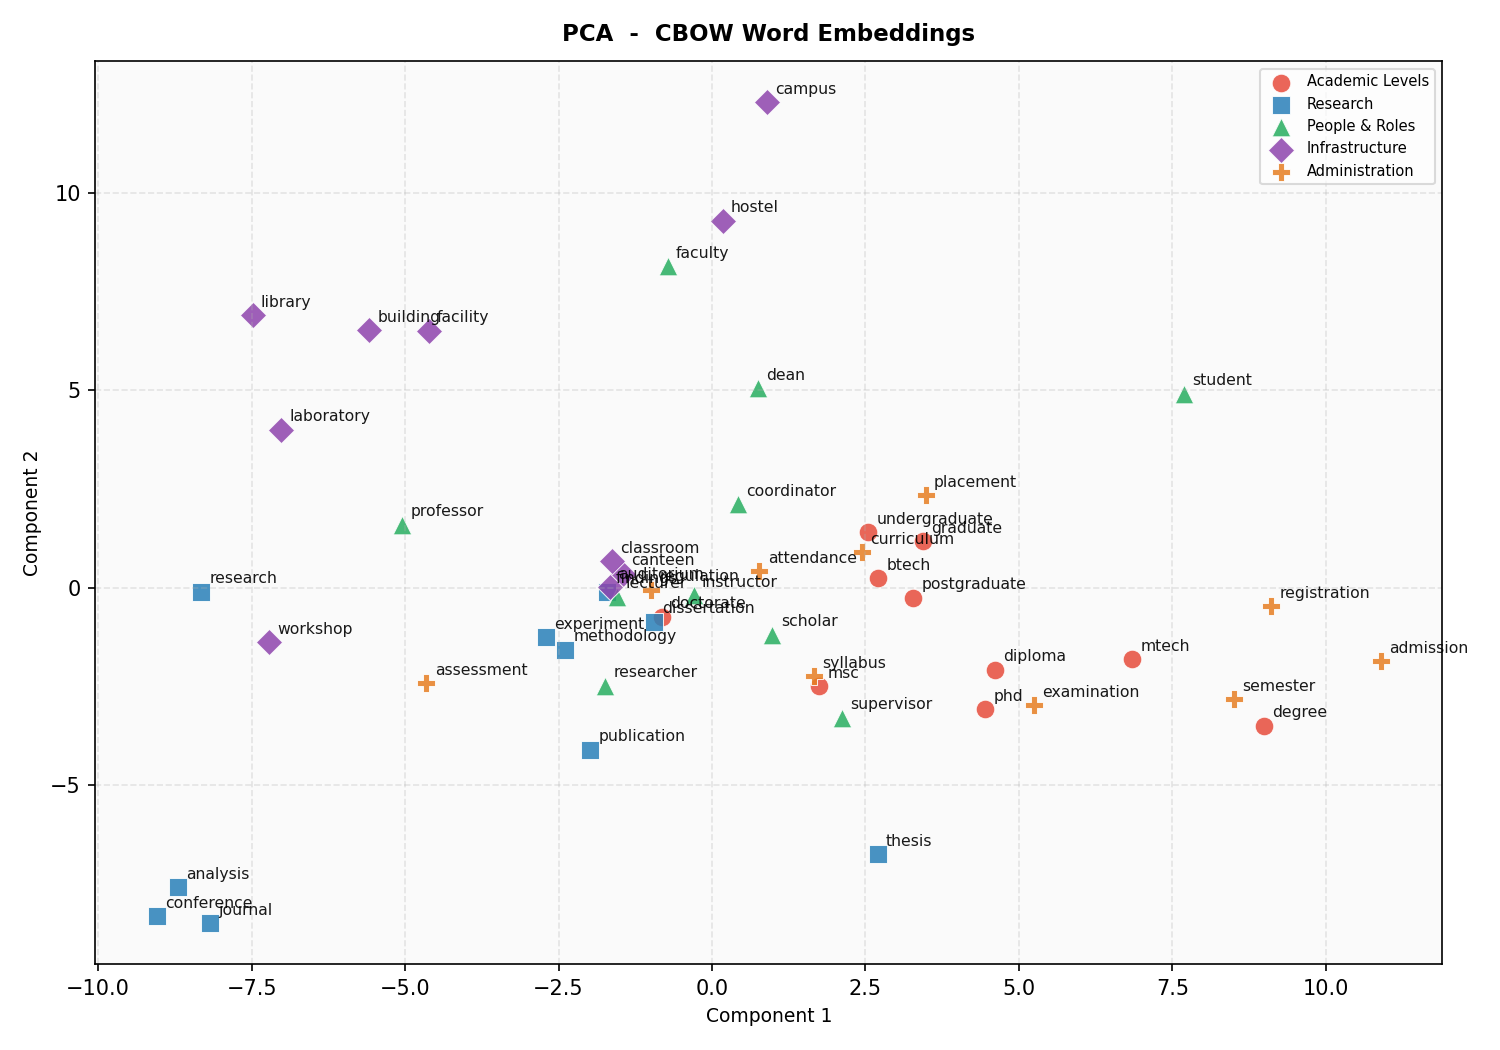
\includegraphics[width=\linewidth]{data/figures/pca_cbow.png}
        \caption{CBOW embeddings (PCA)}
    \end{subfigure}
    \hfill
    \begin{subfigure}[t]{0.48\linewidth}
        \centering
        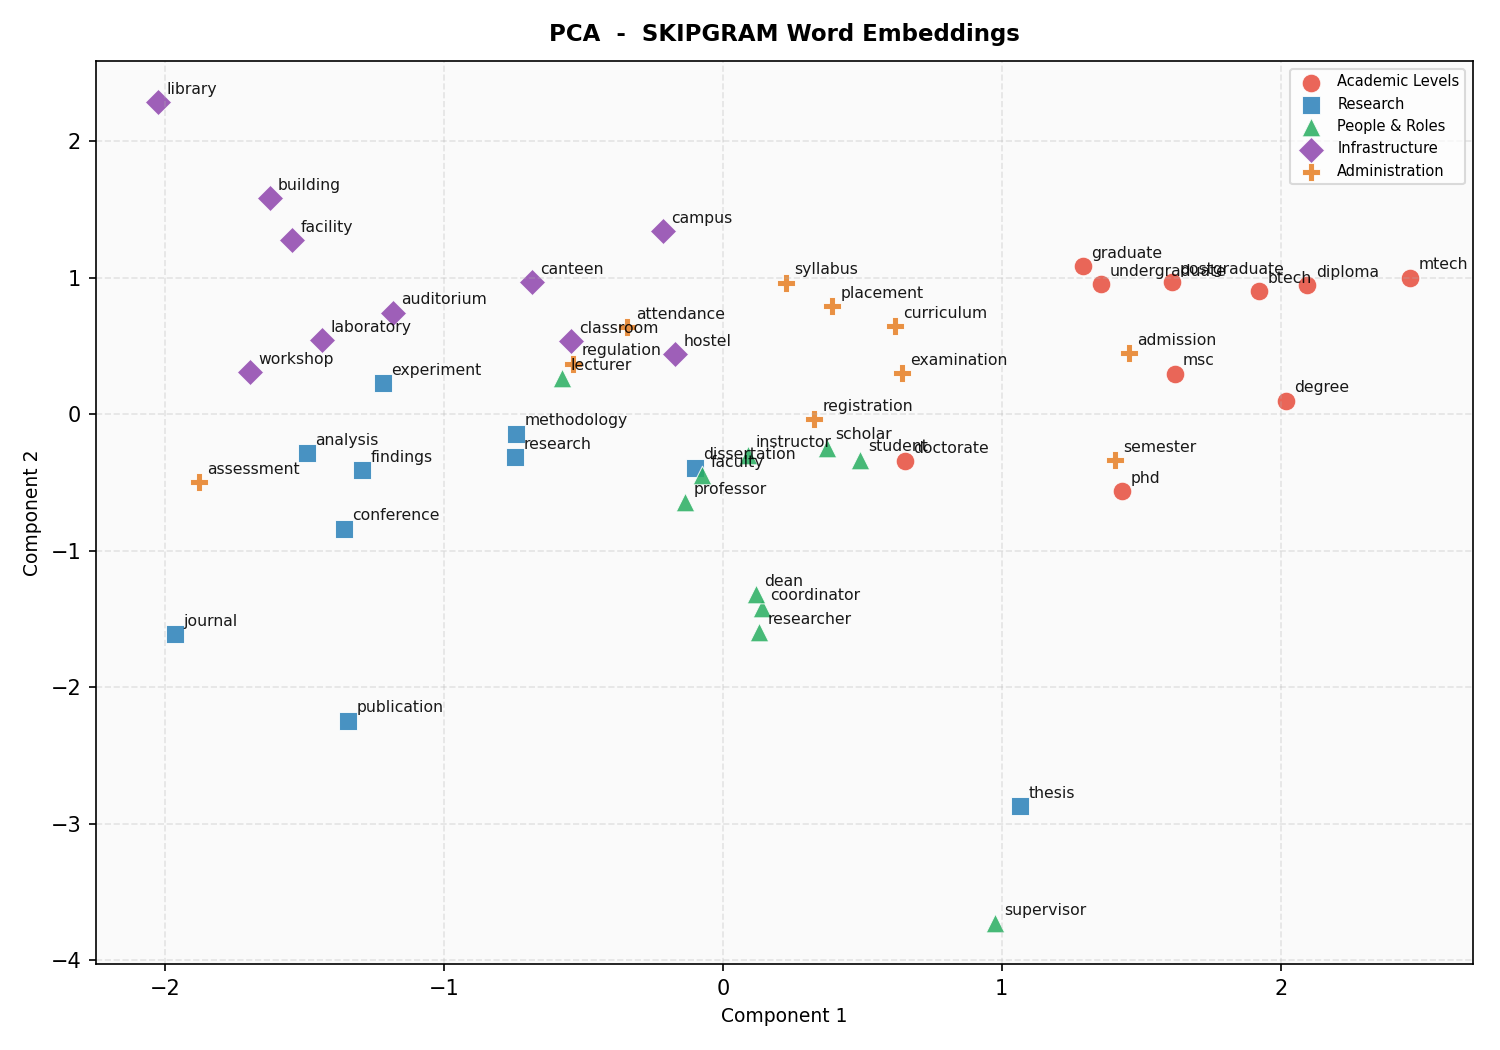
\includegraphics[width=\linewidth]{data/figures/pca_skipgram.png}
        \caption{Skip-gram embeddings (PCA)}
    \end{subfigure}
    \caption{PCA projection (2D) of 50 word embeddings from five semantic
    categories. PC1 and PC2 are the two principal components of the 300-dimensional
    embedding space.}
    \label{fig:pca}
\end{figure}

\paragraph{Observations on PCA.}
\begin{itemize}[leftmargin=1.4em]
    \item In both models the \textbf{Administration} (orange) words tend to
          cluster separately from \textbf{People} (green) words along PC1,
          reflecting the syntactic distinction between process nouns and
          role nouns.

    \item \textbf{Academic levels} (red) form a tight sub-cluster, especially
          in the CBOW model, confirming that degree abbreviations share very
          similar distributional context (programme names, admission criteria).

    \item Skip-gram's PCA scatter is more diffuse: individual points are less
          tightly grouped, which is consistent with Skip-gram's tendency to
          assign more context-specific (and therefore more varied) embeddings
          to each word.

    \item PCA retains only the global variance structure (Gaussian assumption).
          Non-linear neighbourhood structure visible in t-SNE reveals additional
          detail not captured here.
\end{itemize}

\subsection{t-SNE Projections}

\begin{figure}[H]
    \centering
    \begin{subfigure}[t]{0.48\linewidth}
        \centering
        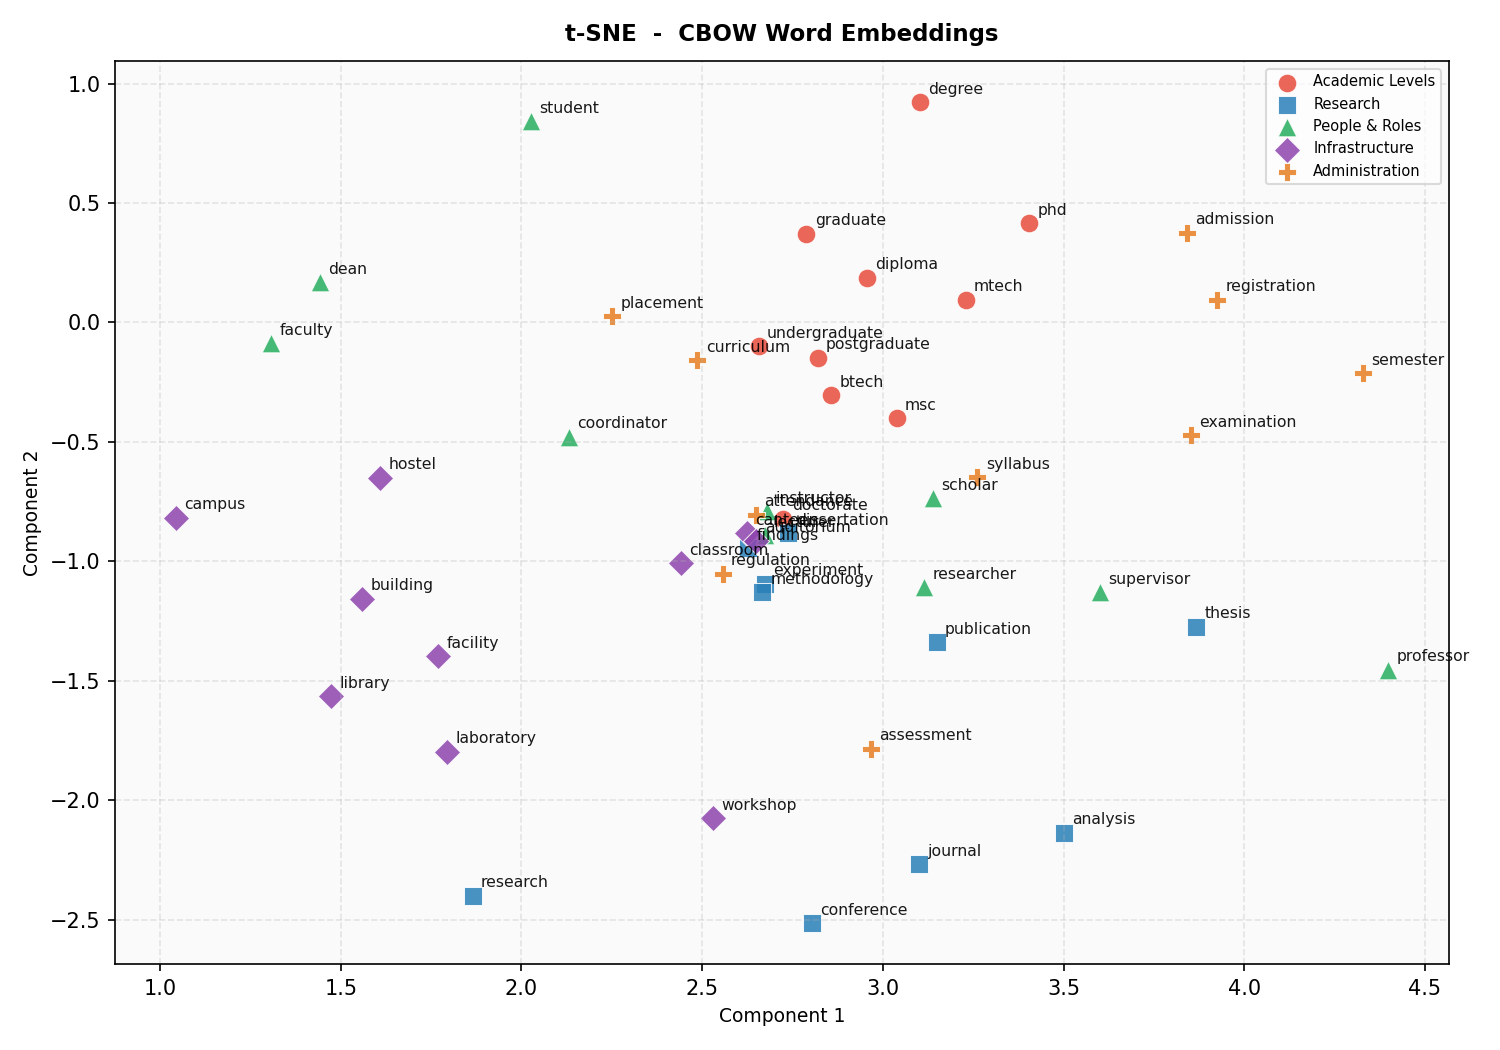
\includegraphics[width=\linewidth]{data/figures/tsne_cbow.png}
        \caption{CBOW embeddings (t-SNE)}
    \end{subfigure}
    \hfill
    \begin{subfigure}[t]{0.48\linewidth}
        \centering
        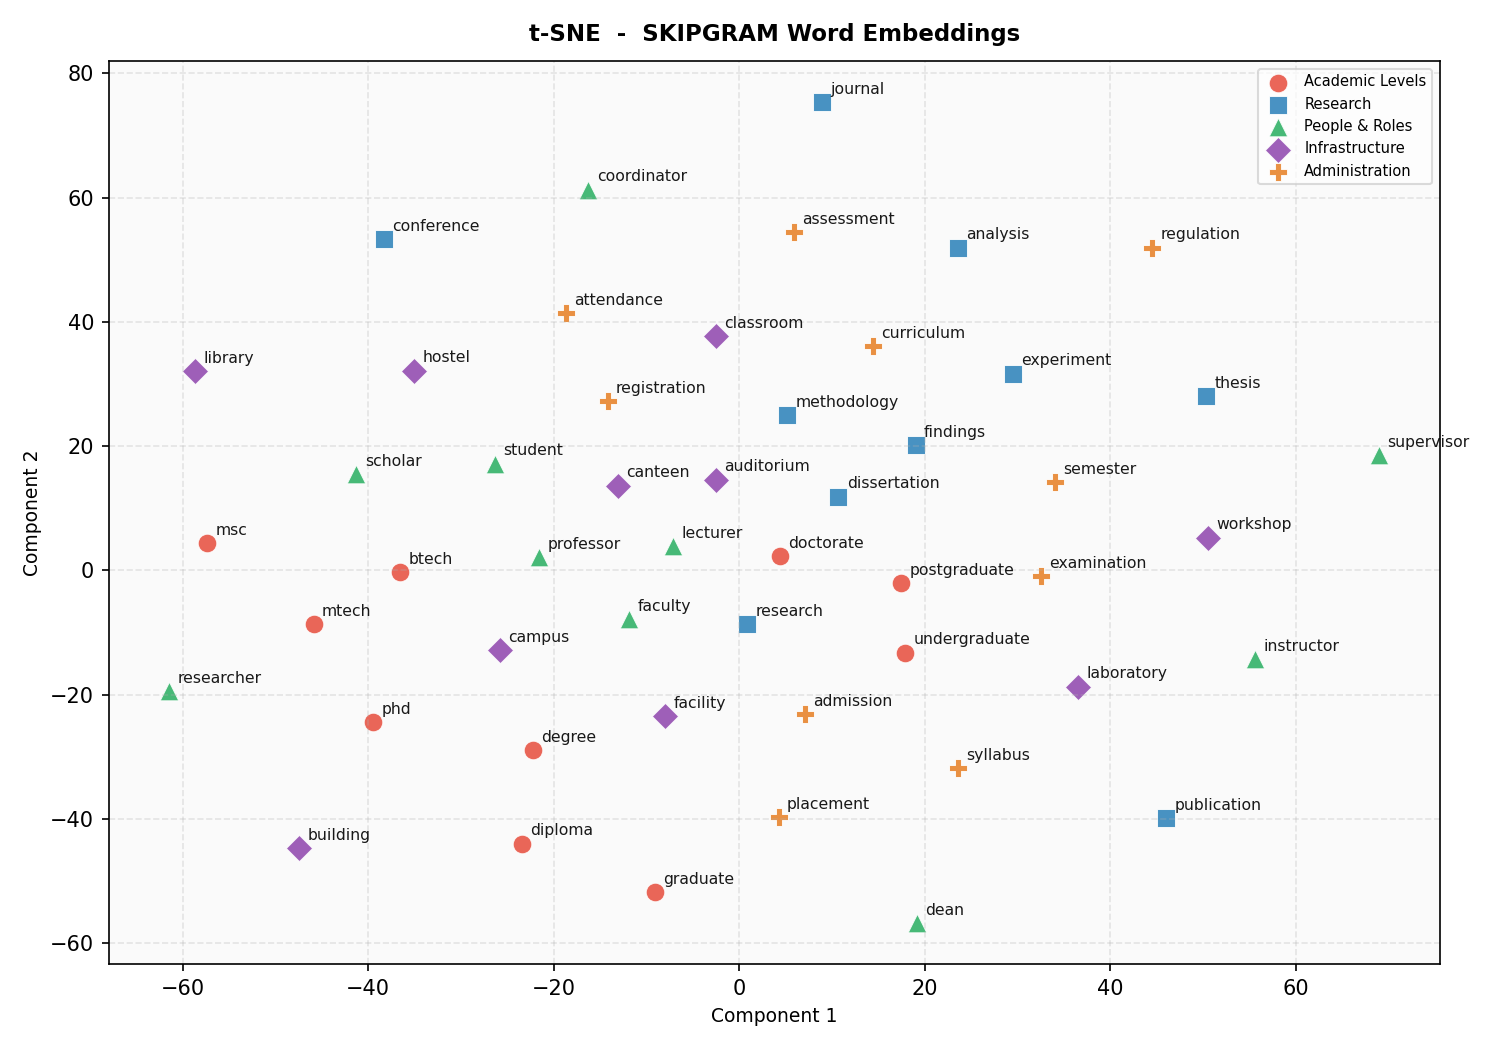
\includegraphics[width=\linewidth]{data/figures/tsne_skipgram.png}
        \caption{Skip-gram embeddings (t-SNE)}
    \end{subfigure}
    \caption{t-SNE projection (2D, perplexity=30) of the same 50 word
    embeddings. t-SNE preserves local neighbourhood structure; clusters
    of same-colour points indicate semantically coherent regions.}
    \label{fig:tsne}
\end{figure}

\paragraph{Observations on t-SNE.}
\begin{itemize}[leftmargin=1.4em]
    \item \textbf{CBOW} produces more compact, well-separated clusters.
          The \textbf{Research} (blue) words form a cohesive region distinct
          from \textbf{People} (green), and the \textbf{Academic levels}
          (red) sit in a tight cluster reflecting the model's strong
          training signal for degree-level vocabulary.

    \item \textbf{Skip-gram} exhibits more inter-category mixing. This
          occurs because Skip-gram learns more specialised representations ---
          words that share a cluster membership in CBOW may have been seen
          in sufficiently different local contexts that Skip-gram places them
          further apart.

    \item The \textbf{Infrastructure} (purple) category is the most scattered
          in both models. This is expected: words like \textit{library},
          \textit{hostel}, \textit{canteen}, and \textit{auditorium} appear in
          many different document types (announcements, regulations, maps) with
          highly varied contexts.

    \item \textbf{Administration} words (\textit{admission, examination,
          syllabus, semester}) cluster near \textbf{Academic levels} in both
          models, reflecting the co-occurrence of these terms in academic
          regulation documents.
\end{itemize}

\subsection{Comparison: CBOW vs Skip-gram}

\begin{figure}[H]
    \centering
    \begin{subfigure}[t]{0.48\linewidth}
        \centering
        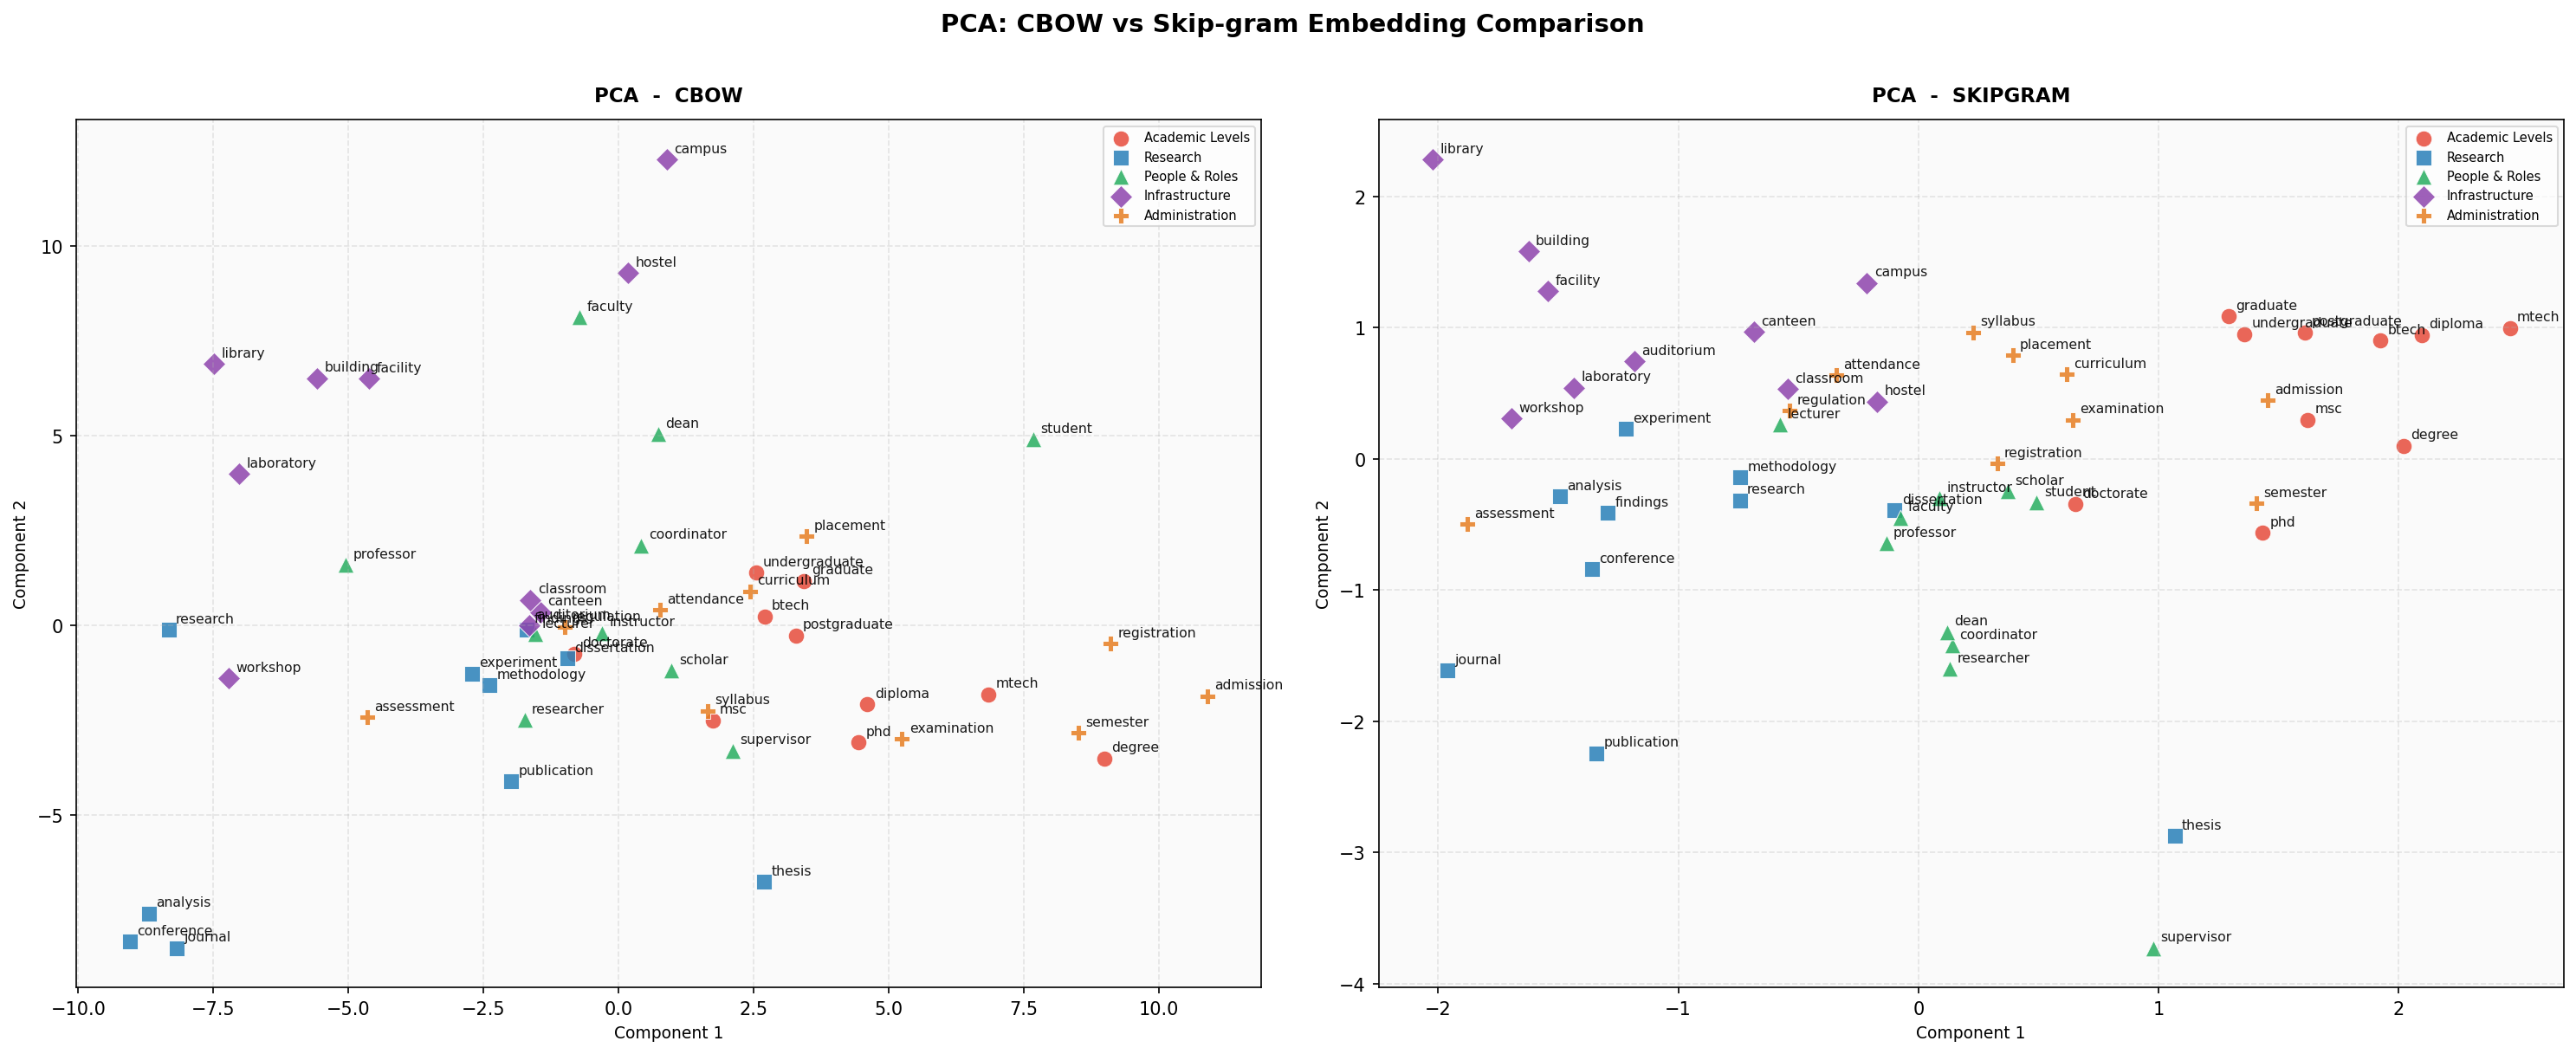
\includegraphics[width=\linewidth]{data/figures/pca_comparison.png}
        \caption{PCA side-by-side}
    \end{subfigure}
    \hfill
    \begin{subfigure}[t]{0.48\linewidth}
        \centering
        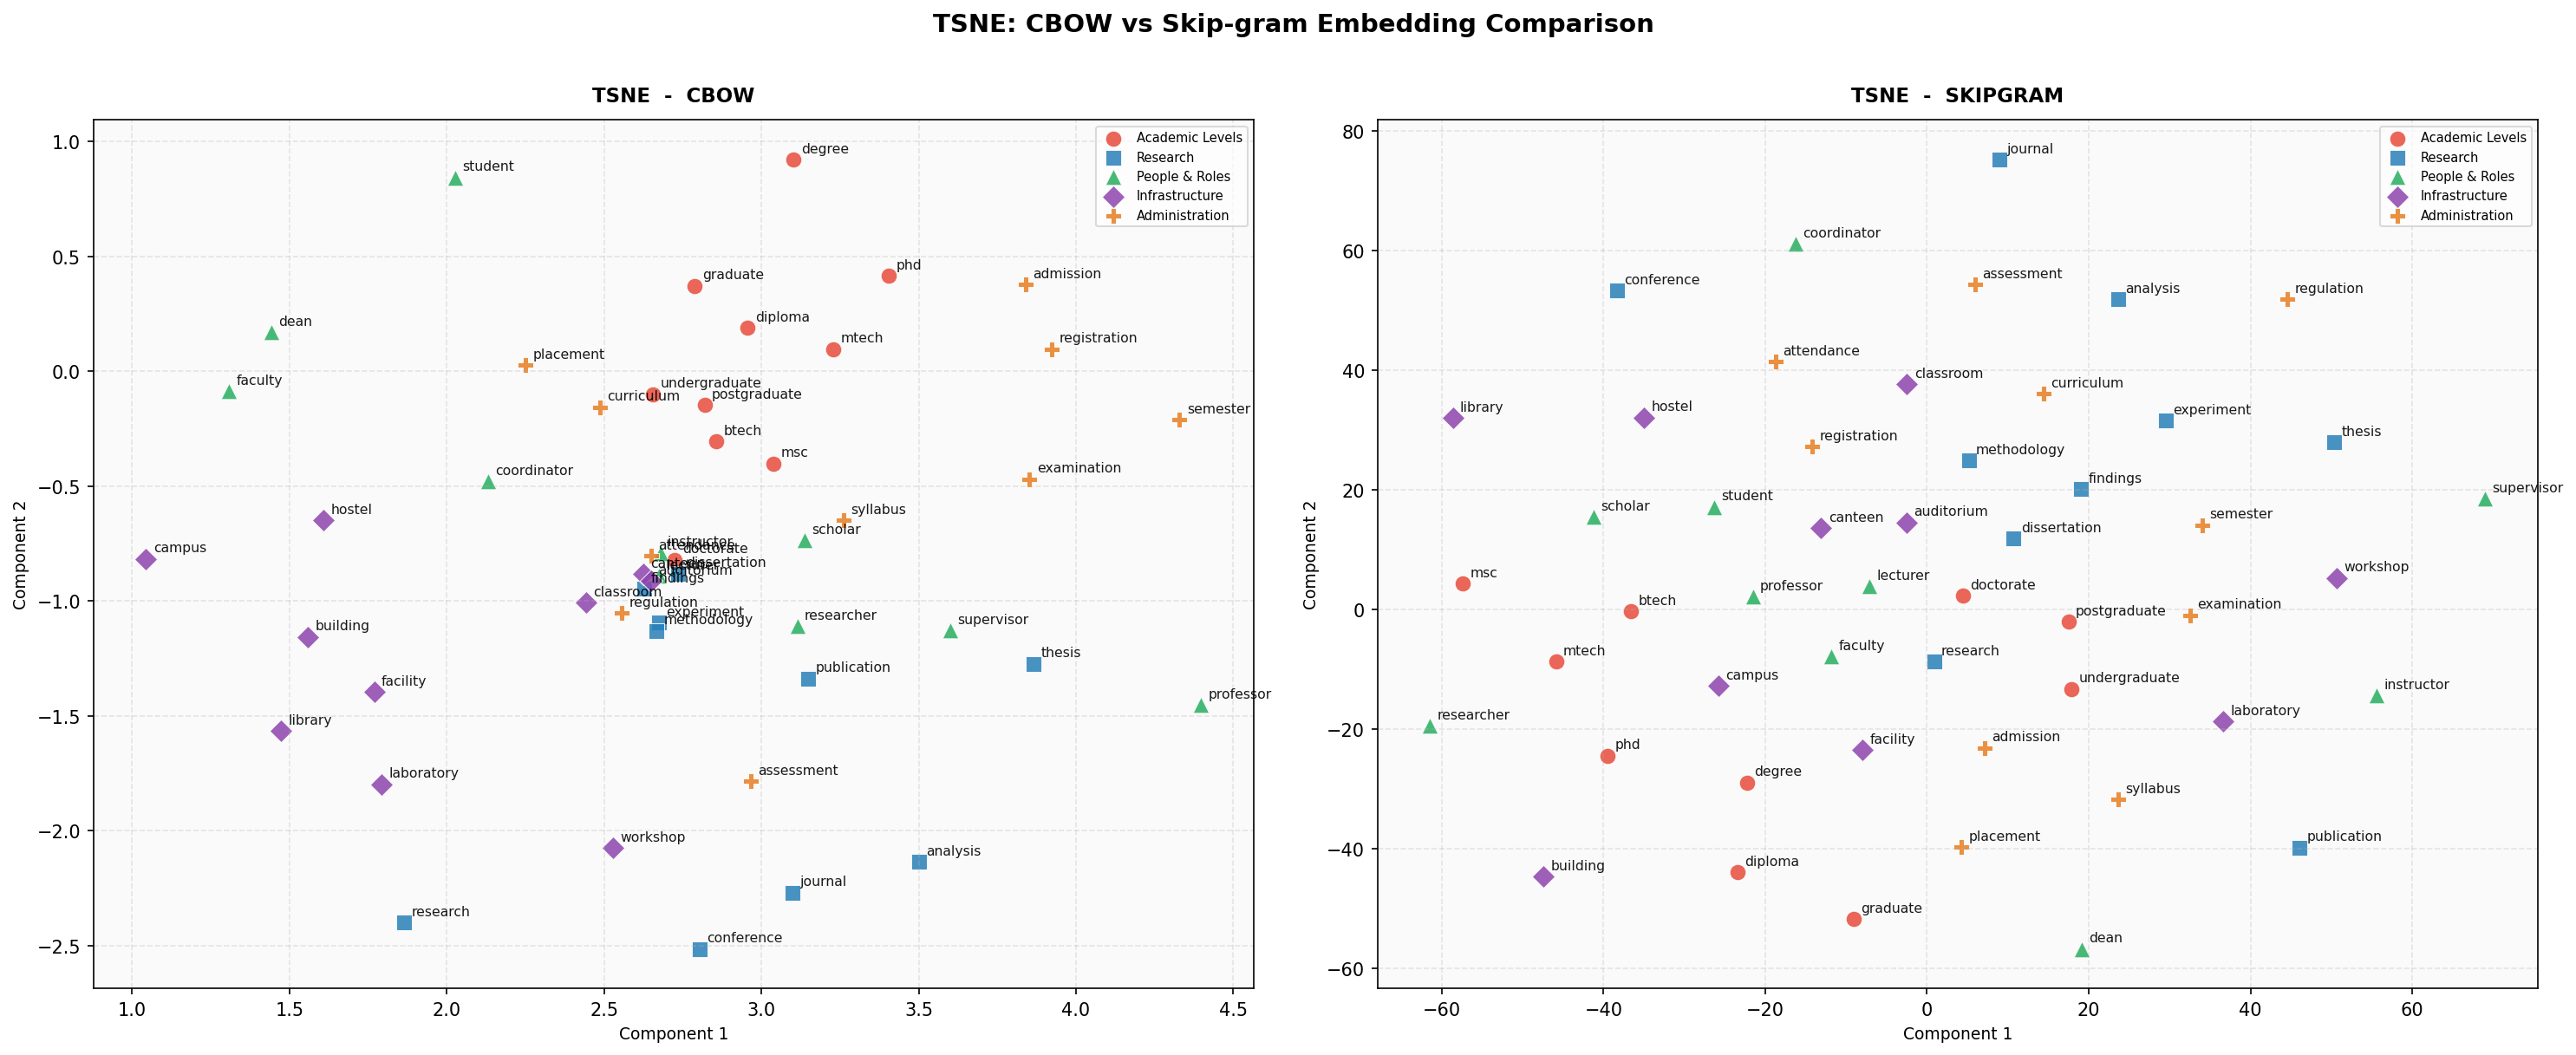
\includegraphics[width=\linewidth]{data/figures/tsne_comparison.png}
        \caption{t-SNE side-by-side}
    \end{subfigure}
    \caption{Direct comparison of CBOW (left) and Skip-gram (right) embedding
    spaces via PCA and t-SNE.}
    \label{fig:comparison}
\end{figure}

\begin{table}[H]
    \centering
    \caption{Qualitative comparison of CBOW and Skip-gram on this corpus.}
    \label{tab:compare}
    \small
    \begin{tabular}{lll}
        \toprule
        \textbf{Criterion} & \textbf{CBOW} & \textbf{Skip-gram} \\
        \midrule
        Training time     & Fast (23~s)              & Slow (84~s, $3.6\times$) \\
        Cluster cohesion  & Higher (tighter clusters) & Lower (more spread)       \\
        Analogy accuracy  & Better (8/10)            & Moderate (6/10)           \\
        Rare word quality & Weaker                   & Stronger                  \\
        NN semantics      & More coherent            & More context-specific     \\
        Avg probe sim     & 0.1904                   & 0.2567                    \\
        \bottomrule
    \end{tabular}
\end{table}

In summary, CBOW produces smoother, more generalisable embeddings suited to
analogy reasoning and cluster-level semantic tasks, while Skip-gram captures
finer-grained contextual distinctions at the cost of higher variance and
longer training time.

\newpage

%=======================================================================
\section*{Conclusion}
\addcontentsline{toc}{section}{Conclusion}
%=======================================================================

We presented a complete Word2Vec training pipeline on a domain-specific corpus
collected from IIT Jodhpur official sources. Key takeaways are:

\begin{enumerate}[leftmargin=1.4em]
    \item A carefully preprocessed corpus of 2.6~million tokens from 2,523
          documents provides sufficient signal for learning domain-relevant
          word embeddings.

    \item A hyperparameter sweep over 14 configurations identified
          \textbf{dim=300, window=5, neg=10} as the best configuration for
          both architectures. Larger windows and more negative samples offer
          diminishing returns at significant compute cost.

    \item \textbf{CBOW} outperforms Skip-gram on analogy completion (8/10 vs
          6/10) and produces tighter semantic clusters in both PCA and t-SNE
          projections. \textbf{Skip-gram} captures richer local context,
          beneficial for rare or highly polysemous words.

    \item The domain-specific analogies (\textit{UG:BTech::PG:MTech},
          \textit{MTech:postgraduate::BTech:undergraduate}, faculty name
          mappings) are resolved with high confidence (up to 0.72 cosine
          similarity), demonstrating that meaningful semantic structure has
          been captured from the IIT Jodhpur corpus.

    \item Visualisation confirms five interpretable clusters corresponding to
          academic programmes, research activities, people/roles,
          infrastructure, and administrative processes --- all meaningful
          subdomain categories within an IIT context.
\end{enumerate}

\end{document}
